
\begin{figure*}[!t]
\centering
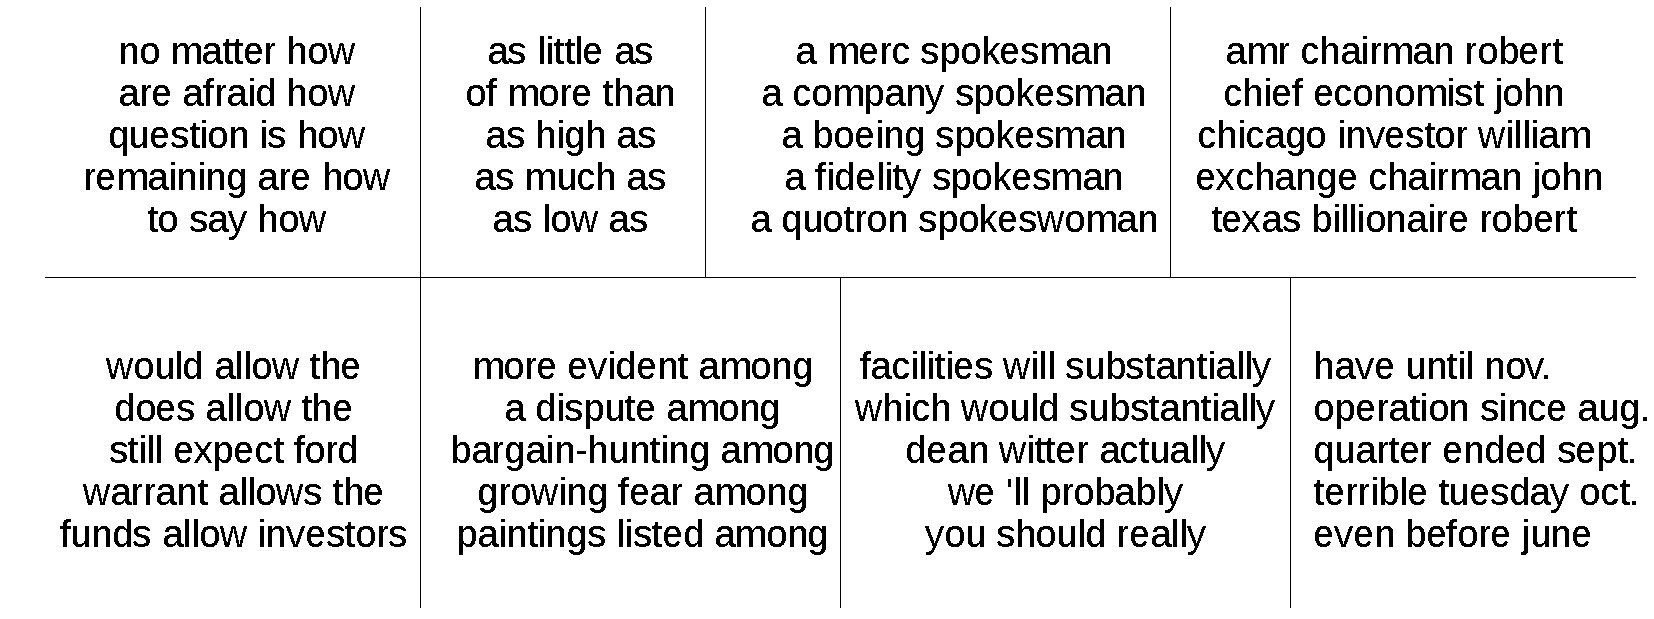
\includegraphics[width=\textwidth]{figures/kernels.pdf}
\centering
\caption{Some example phrases that have highest activations for 8 example kernels (each box), extracted from the validation set of the Penn Treebank. Model trained with 256 kernels for 256-dimension word vectors.}  
\label{fig:kernels}
\end{figure*}

In what follows, we obtain insights into the inner workings of the CNN by looking into
the linguistic patterns that the kernels learn to extract and also studying
the temporal information extracted by the network in relation to its prediction capacity.

\paragraph{Learned patterns} 
To get some insight into the kind of patterns that each kernel is
learning to detect, we fed trigrams from the validation set of the
Penn Treebank to each of the kernels, and extracted the ones that most
highly activated the kernel. Some examples are shown in
Figure~\ref{fig:kernels}. Since the word windows are made of
embeddings, we can expect patterns with similar embeddings to have
close activation outputs.
%~ \gbt{inventing wildly, check following} 
This is borne out in the analysis: The kernels specialize in distinct
features of the data, including more syntactic-semantic constructions
(cf.\ the ``comparative kernel'' including \emph{as \dots as}
patterns, but also \emph{of more than}) and more lexical or topical
features (cf.\ the ``ending-in-month-name'' kernel). Even in the more
lexicalized features, however, we see linguistic regularities at
different levels being condensed in a single kernel: For instance, the
``spokesman'' kernel detects phrases consisting of an indefinite
determiner, a company name (or the word \emph{company} itself) and the
word ``spokesman''. We hypothesize that the convolutional layer adds
an ``I identify one specific feature, but at a high level of
abstraction'' dimension to a feed-forward neural network, similarly to
what has been observed in image
classification~\cite{krizhevsky2012imagenet}.

%~ We assume that, the
%~ convolutional layers altered the values of word embeddings from
%~ \textbf{globally independent} to \textbf{regional values}. \gbt{I
  %~ don't understand this latter sentence. Pls expand.}

%~ \textbf{Kernel size effect} By increasing the size of convolutional
%~ kernels, we want the kernels to learn longer $n$-gram patterns which
%~ can account more complicated phrases. Empirically, we observe that $3$
%~ and $5$ are the optimal kernel size for all of our experiments in all
%~ corpora (results are almost similar). Enlarging the window leads to
%~ the linear increase in the number of convolutional parameters and
%~ complexity, while we did not experience any improvement in
%~ perplexity. Possibly changing the window size requires the
%~ corresponding change in stride and padding, because at stride $= 1$,
%~ two neighbor windows have too much similar content.

%~ \textbf{Multi-layer convolution} \gbt{Why is this in the analysis
  %~ section? It belongs to the experiments section, right?}  With that
%~ interpretation \gbt{What interpretation?}, each convolutional layer is
%~ able to re-estimate embeddings at regional levels \gbt{?}. Therefore,
%~ additional convolutional layers can be applied on top of each other in
%~ order to connect local features, which has shown to be useful in the
%~ context in sentence representation~\cite{Kalchbrenner2014conv}. For
%~ language modeling, however, the performance of the models actually
%~ decreases with the number of layers (see
%~ Table~\ref{tab:ptblayers}). One reason could be the fact that language
%~ modelling contexts are mostly incomplete sentences, with a different
%~ nature than the complete sentences used for sentence
%~ representation. Moreover, stacking convolution layers can make the
%~ whole convolution block become too specific, in that it tries to
%~ remember the exact context in the training data. This may help explain
%~ why increasing the convolutional depth is not suitable for this
%~ particular problem, although further research is needed to test this
%~ claim.



% \gbt{This table was repeated, commenting it out just in case.}
% \begin{table}[tb]
%   \centering
%   \begin{tabular}{|c|c|c|}
%     \hline
%     Model & V & T\\
%     \hline 
%     Baseline ($k=128$) & 114 & 109 \\
%     +CNN ($1$ layer) & 102 & \textbf{97}\\
%     +CNN ($2$ layers) & 113 & 108 \\
% 	+CNN ($4$ layers) & 130 & 124 \\
%     \hline
%   \end{tabular}
% \caption{Performance on the Penn Treebank with different layers.}
% \label{tab:ptblayers}
% \end{table}


\begin{figure}[t]
	\centering
	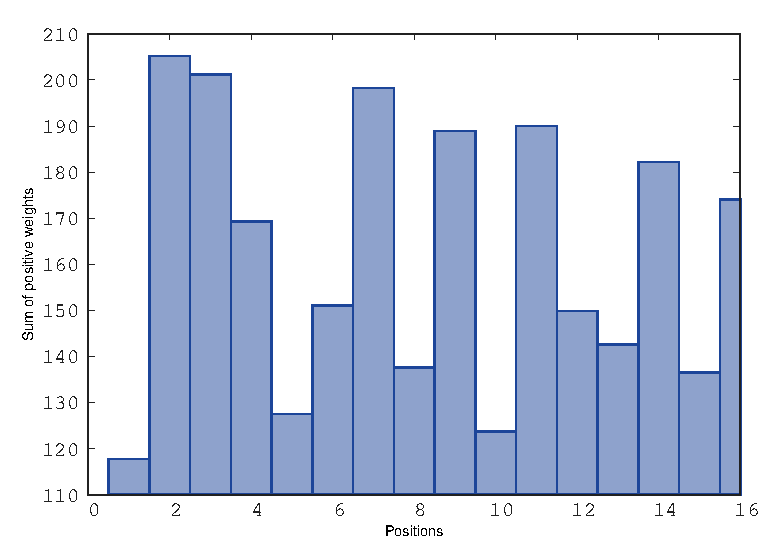
\includegraphics[width=\columnwidth]{figures/weight_dist.eps}
	\caption{The distribution of positive weights over context positions, where 1 is the position closest to the predicted word.}  
	\label{fig:weight-dist}
\end{figure}



\paragraph{Temporal information} To the best of our knowledge, the
longest context used in feed-forward language models is
$10$~\cite{hai2012measuring}, where no significant change in terms of
perplexity was observed for bigger context sizes, even though in that
work only same-sentence contexts were considered. In our experiments, we
use a larger context size of 16 while removing the sentence boundary limit
(as commonly done in $n$-gram language models) such that the network
can take into account the words in the previous sentences.

% We check whether our model \gbt{which version? And how
  %~ are the kernel values combined? E.g. what does the fact that the
  %~ number of active weights at position 3 is much smaller mean, is it
  %~ some effect of choosing kernel size 3? (but then what happens with
  %~ kernel 5?)} does profit from the information in the whole context
%~ through the following experiment:
To analyze whether all this information was effectively used,
 we took our best model, the CNN-NIN-COM model with
embedding size of 256 (fourth line, second block in
Table~\ref{tab:result}), and we identified the weights in the model
that map the convolutional output (of size $n \times k$) to a lower
dimensional vector (the ``mapping'' layer in
Figure~\ref{fig:simpleconv}). Recall that the output of the convolutional layer is
a matrix indexed by time step and kernel index representing the activation of
the kernel when convolved with a window of text centered around the given time step. Thus,
output units of the above mentioned mapping predicate over an ensemble of kernel activations for
each time-step . We can identify the
patterns that they learn to detect by extracting the time-kernel combinations
for which they have positive weights (since we have ReLU
activations, negative weights are equivalent to ignoring a
feature). 
First, we asked ourselves whether these units tend to be more
focused on the time-steps closer to the target or not. To test this,
we calculated the sum of the positive weights for each position in time using an average of the mappings that correspond to each output unit. %, even when the distribution of weights cannot allow us to obtain an attentional behaviour similar to the Memory Network~\cite{sukhbaatar2015end}.
The results are shown in
Figure~\ref{fig:weight-dist}. As could be expected, positions that are
close to the token to be predicted have many active units (local
context is very informative; see positions 2-4). However,
surprisingly, positions that are actually far from the target are also
quite active (see positions 10-14, with a spike at 11). It seems like the
CNN is putting quite a lot of effort on characterizing long-range
dependencies. %\newgk{This is not true, right?} Overall, the extent of activeness gradually reduces from the closest to the farthest position, which is in line with the previous work~\cite{hai2012measuring}. 
%Also, the effect of convolution is also reflected here, when the weights in the middle seem to fluctuate with the stride of the convolution. 

\begin{figure}[t]
	\centering
	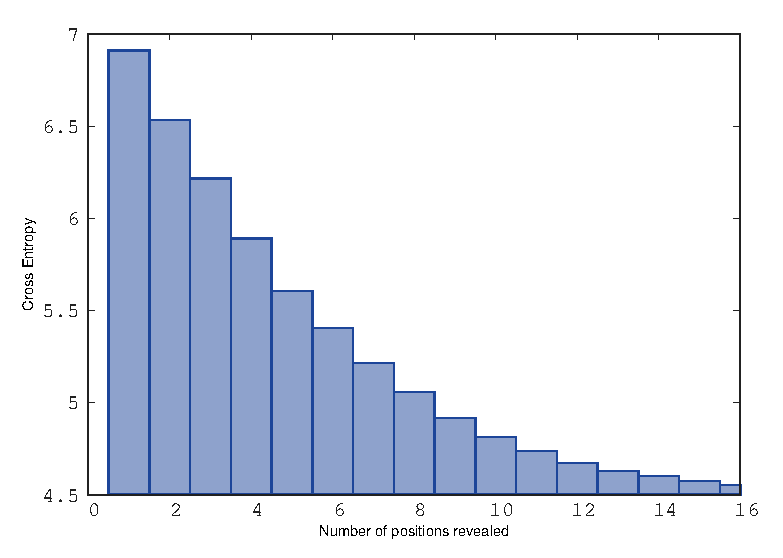
\includegraphics[width=\columnwidth]{figures/ppl_positions.eps}
	\caption{Perplexity change over position, by incrementally revealing the Mapping's weights corresponding to each position.}  
	\label{fig:position}
\end{figure}

Next, we checked that the information extracted from the positions
that are far in the past are actually used for prediction. To measure
this, we artificially lesioned the network so it would only read the
features from a given range of timesteps 
%\newgbt{check following}
(words in the context).  To lesion the network we manually masked the
weights of the mapping that focus on times outside of the target range
by setting them to zero. We started using only the word closest to the
final position and sequentially unmasked earlier positions until the
full context was used again. The result of this experiment is
presented in Figure~\ref{fig:position}, and it confirms our previous
observation that positions that are the farthest away contribute to
the predictions of the model. The perplexity drops dramatically as the
first positions are unmasked, and then decreases more slowly. However,
the last few positions still contribute to the final
perplexity. Indeed, the decrease almost follows a power-law
distribution, in which the perplexity decreases whenever we unmask a new position according to the following equation.

\begin{equation}
f(x) = 10e3 \times x^{-0.9}
\end{equation}



%~ \gk{Don't have the numbers here. Can you check if this is about right?}.


%\begin{itemize}
%\item First, we identified the weights in the hidden layer that map
%  the convolutional output from ($n \times k$)to a lower dimension
%  ($2 \times k$).
%\item Second, we masked the weights with zero, and then incrementally
%  unmasked the weights corresponding to each position, starting with
%  the one closest to the predicted word.
%\end{itemize}

%~ \gbt{Make font of axes in Figs 5, 6 larger (at least as large as
  %~ caption size). Also make ``plus'' signs larger. Why is there no
  %~ datapoint at position 16?}
%Figure~\ref{fig:position} records the perplexity change when unmasking
%the weights corresponding to each position. The perplexity drops
%dramatically in the first few positions, and then decreases more
%slowly; however, the last few positions still contribute to the final
%perplexity. 

%We also extracted the average number of positive weights on each position
%(Figure~\ref{fig:weight-dist}),indicating the
%number units that are active at each position. 
%  which showed that weights assigned for
% the last positions are quite active, while the most active area
% belongs to the closest positions to the predict words.
%~ \gbt{I'm inventing wildly in what follows, pls check.}  



%~ \textbf{Sampling}
